\documentclass[11pt]{article}
\usepackage[a4paper,margin=2.4cm]{geometry}
\usepackage[T1]{fontenc}\usepackage[utf8]{inputenc}
\usepackage{booktabs,graphicx}
\title{sized\_hdpe\_500N\\\large Hybrid Rocket Motor Design Report (HyProp)}
\author{Generated by HyProp}
\begin{document}\maketitle
\section{Mission Requirements}
Required thrust: 500 N; total impulse: 4e+03 N\,s; design altitude: 1e+03 m; safety factor: 1.5.
\section{Inputs and Assumptions}
Oxidizer: N2O at 293 K (self-pressurized). Fuel: HDPE. Injector: 4$\times$1.65 mm, $C_d$=0.6 (SPI). Efficiencies: $\eta_{c^*}$=0.95, nozzle extra $\eta$=0.9673, divergence half-angle 15.0$^\circ$.
\section{Grain and Chamber Geometry}
Geometry: cylindrical; length 508 mm; outer diameter 43.1 mm; port parameters: {'initial_diameter_m': 0.025997243922216768}. Tank: 2.4 L, 1.66 kg oxidizer.
\section{Transient Simulation}
Burn time 17 s; total impulse 4.08e+03 N\,s; peak thrust 604 N; peak chamber pressure 38.2 bar; propellant used 2.05 kg; mean delivered $I_{sp}$ 203 s. Events: liquid runout at 7.24 s; pressure decay at 17.04 s.
\section{Representative Operating Points}
The plain time average is misleading for blowdown motors: it understates thrust by 51\% and chamber pressure by 48\% versus the impulse-weighted point. All design modules therefore use the weighted points below.
\begin{table}[h!]\centering\caption{Representative operating points vs plain time average (SI units).}
\resizebox{\textwidth}{!}{%
\begin{tabular}{lrrrrrrrrrrrrrrrrrrrrrrrrrr}
\toprule
 & pc\_max & pc\_max\_time\_s & thrust\_max & thrust\_max\_time\_s & t\_c\_max & t\_c\_max\_time\_s & cstar & d\_port & g\_flux & gamma & impulse & isp & m\_fuel & m\_ox & m\_ox\_liquid & mdot\_fuel & mdot\_ox & mdot\_total & of & p\_tank & pc & rdot & t\_c & t\_tank & thrust & web \\
\midrule
peak\_performance & 3824937.316700 & 0.000000 & 604.445500 & 0.000000 & 3242.041900 & 0.000000 & 1533.595100 & 0.026000 & 426.615500 & 1.249800 & 12.088900 & 235.490700 & 0.458600 & 1.661100 & 1.604200 & 0.035300 & 0.226500 & 0.261700 & 6.418600 & 5060128.300900 & 3824937.316700 & 0.000900 & 3242.041900 & 293.150000 & 604.445500 & 0.000000 \\
impulse\_weighted & NaN & NaN & NaN & NaN & NaN & NaN & 1487.907000 & 0.031800 & 254.072700 & 1.258100 & 2049.346000 & 220.504200 & 0.324200 & 0.887900 & 0.717300 & 0.034700 & 0.188600 & 0.223300 & 5.360700 & 4122378.712900 & 3196133.940000 & 0.000700 & 2952.310600 & 282.782400 & 493.747700 & 0.002900 \\
heat\_load & NaN & NaN & NaN & NaN & NaN & NaN & 1533.595100 & 0.026000 & 426.615500 & 1.249800 & 12.088900 & 235.490700 & 0.458600 & 1.661100 & 1.604200 & 0.035300 & 0.226500 & 0.261700 & 6.418600 & 5060128.300900 & 3824937.316700 & 0.000900 & 3242.041900 & 293.150000 & 604.445500 & 0.000000 \\
mass\_flow & NaN & NaN & NaN & NaN & NaN & NaN & 1454.966800 & 0.032700 & 227.873700 & 1.258600 & 2283.116500 & 202.787500 & 0.301100 & 0.793100 & 0.631600 & 0.032800 & 0.170900 & 0.203700 & 4.915500 & 3771809.826100 & 2901048.817000 & 0.000700 & 2797.979600 & 273.495200 & 444.096100 & 0.003300 \\
median\_impulse & NaN & NaN & NaN & NaN & NaN & NaN & 1506.145000 & 0.031800 & 249.866500 & 1.258700 & 2049.618200 & 227.058800 & 0.329600 & 0.891300 & 0.698200 & 0.035700 & 0.198100 & 0.233800 & 5.545700 & 4240629.483300 & 3355019.870700 & 0.000700 & 3033.986500 & 285.525400 & 520.518600 & 0.002900 \\
time\_average & NaN & NaN & NaN & NaN & NaN & NaN & 1319.093400 & 0.036300 & 122.973700 & 1.260600 & 3174.141100 & 121.275300 & 0.203400 & 0.424300 & 0.311900 & 0.023900 & 0.096500 & 0.120400 & 2.999400 & 2249226.717400 & 1669919.114600 & 0.000500 & 2165.917900 & 228.286000 & 239.526300 & 0.005100 \\
\bottomrule
\end{tabular}
}\end{table}
\begin{table}[h!]\centering\caption{Burn phases: liquid / transition / gas.}
\resizebox{\textwidth}{!}{%
\begin{tabular}{lrrrrrrrrrrrr}
\toprule
 & t\_start\_s & t\_end\_s & impulse\_ns & impulse\_share & time\_share & mean\_thrust & mean\_pc & mean\_of & mean\_isp & mean\_cstar & mean\_gamma & mean\_t\_c \\
phase &  &  &  &  &  &  &  &  &  &  &  &  \\
\midrule
liquid & 0.000000 & 7.220000 & 3753.757500 & 0.920800 & 0.424200 & 519.905800 & 3350457.261800 & 5.561600 & 226.987300 & 1506.745400 & 1.258500 & 3038.444200 \\
transition & 7.240000 & 7.480000 & 52.018200 & 0.012800 & 0.014100 & 224.065800 & 1617384.014200 & 3.325200 & 179.959300 & 1344.440700 & 1.260400 & 2220.515900 \\
gas & 7.500000 & 17.020000 & 258.502500 & 0.063400 & 0.559300 & 27.296300 & 396599.261400 & 1.046700 & 39.442700 & 1176.051300 & 1.262100 & 1502.630300 \\
\bottomrule
\end{tabular}
}\end{table}
Time share needed to deliver impulse fractions: 50% of $I_t$ in 21.3% of burn time, 75% of $I_t$ in 33.4% of burn time, 90% of $I_t$ in 41.3% of burn time, 95% of $I_t$ in 45.9% of burn time, 99% of $I_t$ in 56.4% of burn time.
\subsection{Recommendations}\begin{itemize}
\item Nozzle design and reported performance: \textbf{impulse-weighted} point (each instant weighted by its contribution to total impulse).
\item Thermal/erosion analysis: \textbf{heat-load} point (maximum of the Bartz $\sim P_c^{0.8}$ proxy).
\item Structural sizing and materials: \textbf{peak-performance} envelope ($P_c$=38.2 bar, $T_c$=3242 K).
\item Injector and feed system: \textbf{mass-flow-weighted} point.\end{itemize}
\section{Nozzle and Performance}
Throat diameter 11.7 mm; expansion ratio 5.02; impulse-weighted $I_{sp}$ 221 s, $c^*$ 1.49e+03 m/s, O/F 5.36.
\section{Figures}
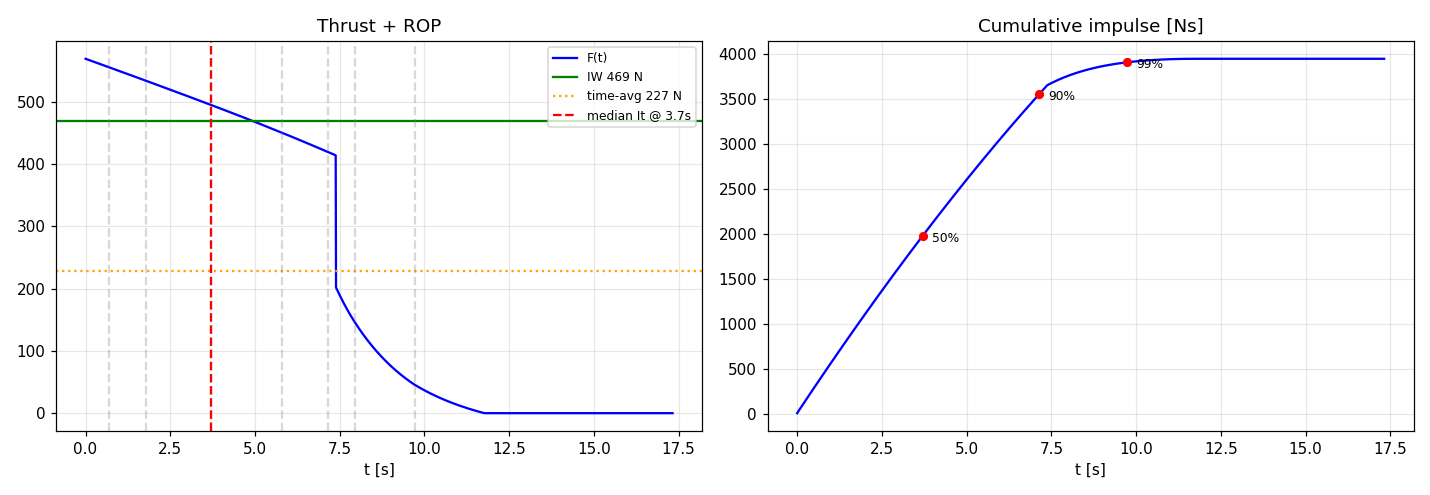
\includegraphics[width=\textwidth]{rop_hdpe_05kN.png}
\section{Validation Note}
Models validated against NASA-CEA-class thermochemistry (Cantera cross-check), HRAP transient benchmark (prusak\_v2) and ESDU 91022/CoolProp N2O properties; see repository README. Empirical coefficients (a, n, $C_d$, $\eta$) require confirmation by fire tests before design freeze.
\end{document}